\chapter{Theoretical Background}
\label{chap:background}

% \thispagestyle{fancy}
This chapter provides the theory essential to understand the major components of the thesis. Prior knowledge of Artificial Neural Networks \cite{theory_ann_wiki} and fundemental concepts of Deep Learning \cite{theory_dl} is assumed.

% TODO -- add the theory of all concepts VAEs NSFRM etc
\section{Preliminary Concepts}
\label{sec:Preliminary}

% TODO -- add the theory of all concepts VAEs NSFRM etc
\subsection{Autoencoder}
Autoencoders are a variant of \acp{ann}, which are designed to learn an identity function that generates the input data sample back. The network has a bottleneck($z$), dividing the network into two parts, an encoder and a decoder as illustrated in fig[\ref{fig:ar_arch}]. The former learns to compress the high demensional input data to a low dimensional intermediate representation, \textit{latent representation}, at the bottleneck. While the latter learns to reconstruct the data from the latent distribution. Thus learning to efficiently compressing the data. 

To put it in other words, in the process of learning to reconstruct the data, the encoder learns to filter the most important features of the given data distribution, so as it preserve the complete properties within the limits of the bottleneck. While the decoder learns more general properties of the distribution which is used along with the compact latent representation from the encoder to fully recover the data distribution. The network is trained to minimize the similarity between the reconstruction and the original data sample. This similarity can be determined by metrics such as \ac{mse}, \ac{l1} or Cross-Entropy loss. 

The idea of an autoencoder dates back to the 80's proposed as a method for pre-training and feature learning \cite{ballard1987modular, rumelhart1985learning}, learnt dimensionality reduction \cite{hinton_dimentionality}. In recent years, autoencoders are most popularly used as generative networks leveraging their ability to learn feature representations in an unsupervised way. Another interesting variant of autoencoders are denoising autoencoders \cite{vincent2008extracting}, where the input is a noised data and the decoder generates original data without noise. This variant is further evolved to accomplish the tasks of image denoising, watermark removal, inpainting, super resolution, colorization, de-colorization and compression \cite{zhang2016colorful, imagedenoisingpaper}. Improved variants of autoencoders that are relant to this thesis are introduced next.  %FIXME add more?

\begin{figure}[!h]
    \centering
    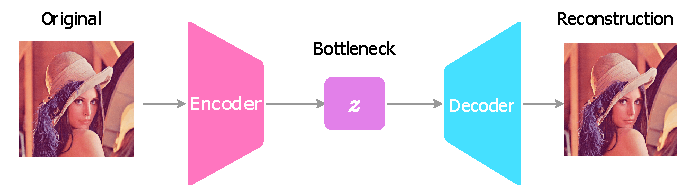
\includegraphics[scale=1]{figures/ae_arch.pdf}
    \caption{Illustration of Autoencoder architecture.}
    \label{fig:ar_arch}
\end{figure}

% TODO -- add the theory of all concepts VAEs NSFRM etc
\subsection{Variational Auto Encoders}


\begin{figure}[!h]
    \centering
    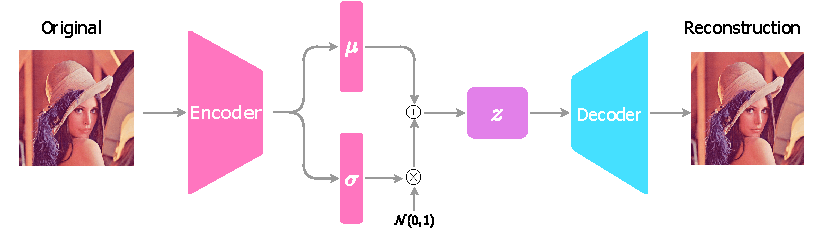
\includegraphics[scale=1]{figures/vae_arch.pdf}
    \caption{Illustration of Variational Autoencoder architecture.}
    \label{fig:vae_arch}
\end{figure}

% TODO -- add the theory of all concepts VAEs NSFRM etc
\subsection{Generative Adversarial Networks}


% TODO -- add the theory of all concepts VAEs NSFRM etc
\subsection{Hybrids}

from the laearned features representations from gans, we can use it as the similarity metric without requireing labels for element wsise similarity metric, cite first v gan paper \cite{autoencoding_beyond_pixels}

\lipsum[1-4] %FIXME

% FIXME -- polish related works
\section{Research Area Introduction}
\label{sec:Research area introduction}

In this section the details of various related works and the state-of-the-art in 3D Human Pose Estimation are presented along with some works in the sibling task of hand pose estimation.

\subsection{Pose from images}
There are numerous works that try to estimate 3D human poses from 2D \ac{rgb} images or 2D joint confidence heatmaps \cite{CameraDistanceAware, poselifter, DistillNRSfM, occlusionVideo}. Most of these methods follow a cascading approach, where an explicit intermediate representation of 2D pose or 2D heatmaps is used.

For example, \cite{CameraDistanceAware} proposes a general framework with 3 networks. Human detection Network, RootNet, PoseNet. Where, the human detection network predicts the region the human is in an image. The RootNet localizes the human's root in the global 3D world. And, the PoseNet predicts the 3D pose of a single person with respect to the root. Where, the root is a fixed reference point of the human body say, pelvis.

The advantage of such top-down frameworks is to divide the task of RGB to 3D into smaller, well-studied sub-tasks. This makes scaling single-person pose estimation algorithms for multi-person pose estimation easy, as the majority of the data available mostly consists of a single person per frame. In addition to it, this approach provides the opportunity to improve certain modules without affecting or having to re-train the other modules of the system.

\subsection{Pose Lifting}

In contrast to the estimating pose from an image, Pose Lifting works such as \cite{poselifter,  amazon1, repnet, c3dpo, unsupervisedAdversarial}, focus on estimating 3D poses from 2D poses alone. Assuming 2D poses from the \ac{sota} methods in 2D \ac{hpe}. These methods include simple linear models as first described in \cite{MartinezHRL17} with a series of fully connected linear layers, and sometimes batch normalization, dropout and, residual connections to regress 3D pose effectively.

\ac{nrsfm} is another promising lifting method that also leverages images along with 2D annotations. \ac{nrsfm} deals with the problem of reconstructing 3D shape (pose/point cloud) and cameras of each projection from a sequence of images with corresponding 2D orthogonal projections (2D keypoints). This approach has been widely used in facial keypoint detection and \cite{deepNRSFM} introduces deep learning variant for the same. Instead of predicting the 3D coordinates of each keypoint/joint of the 3D pose, \cite{DistillNRSfM, c3dpo, deepNRSFM, nrsfm++} predicts the 3D shape and camera pose from 2D pose using this method.

The Pose Lifting approach facilitates to leverage the already well established 2D \ac{hpe} models that are trained on enormous and diverse labelled data. Thus demanding lesser training data for 3D pose estimation than it would need when learning from images. Since these networks do not have large convolution layers they are less computationally inexpensive for both training and inference on edge computing units. Moreover, the 2D and 3D pose data usually can be entirely loaded on to GPU further accelerating the training procedure. Thus addressing the critical problem that hinders scalability of 3D \ac{hpe} models and also helps to develop better modular systems by combining the best of Pose Lifting networks with the best of 2D \ac{hpe}. However, due to the inherent ambiguity in lifting pose to 3D and as the images are not captured with orthogonal cameras, reprojection of 3D pose will vary from the ground truth, it is challenging to match the performance of models trained on 3D ground truth.

\subsection{Non-Supervised Learning}

The standard way to train 3D/2D \ac{hpe} is by minimizing the distance between the predicted 3D/2D pose and its corresponding ground truth. The area of 2D \ac{hpe} is well established and matured with reliable systems deployed in the real world. This was made possible with the high volume of images from diverse settings and the reasonable ease of manual labelling of 2D poses. On the other hand, labelling 3D pose manually is not practical. Though single-person datasets such as Human3.6M \cite{H3.6}, Human Eva \cite{HumanEva} and, multi-person datasets such as CMU Panoptic \cite{cmuPanoptic} provide 3D pose ground truth. They are obtained using \ac{mocap} systems which are only limited to indoors or cannot be directly adapted to outdoor environments where the majority of the use cases exist fig[\ref{fig:h36_mocap}]. It is also worth mentioning JTA(Joint Track Auto) dataset \cite{JTA} that is made using the GTA(Grand Theft Auto) game engine which is technically scalable with its own limitations. But datasets from simulations come with the difficulty of domain adaptation to be transferable to the real world.

\begin{figure}[!h]
    \centering
    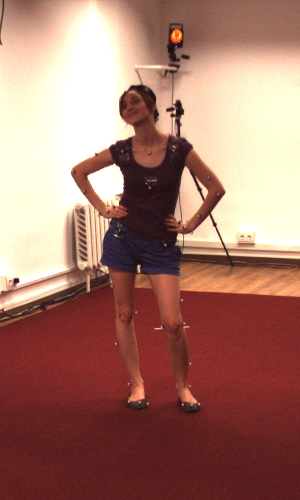
\includegraphics[width=30mm]{figures/h36_mocap.png}
    \caption{Image from Human3.6 Dataset \cite{H3.6} of subject wearing \ac{mocap} markers}
    \label{fig:h36_mocap}
\end{figure}

To overcome this bottleneck, \cite{unsupervisedAdversarial} proposes unsupervised training of a generative adversarial network by projecting the predicted 3D pose back to 2D and minimizing its distance with the input 2D pose. And further training a discriminator to distinguish the real 2D pose from the projected poses. Thus removing the need for any explicit 3D annotations besides 2D poses that are either manually labelled or obtained using 2D \ac{hpe} models. RepNet \cite{repnet}, trains an adversarial network without 2D-3D correspondences in a weakly supervised manner. Moreover, it also does not require camera parameters to project the 3D pose but learns to predict them. Thus enabling better generalization to more diverse data with unknown cameras and poses.

To test the maximum capability of Pose Lifting networks, \cite{amazon1} proposes a combination of unsupervised and adversarial learning that mainly leverages the property of \textit{plane-invariance}. It is the property that 2D projections of a 3D pose from different camera viewpoints, when lifted should produce identical and the original 3D pose. In this method, the predicted 3D pose is rotated in random angles and is reprojected to 2D in a different \ac{pov}. A discriminator is then used to evaluate if this new 2D pose is in the possible pose distribution which is learnt from 2D pose datasets alone. These steps are redone in reverse order to obtain the original 2D input. This cycle provides three intermediate representations of the single 2D input that the models learn from. Additionally, this approach exploits the temporal consistency in the datasets as well as integrates a domain adaptation network to learn from different datasets and distributions to achieve comparable results to that of the methods that require more supervision.


\subsection{Multimodal Representation Learning}
\label{section:multimodal_representation_learning}
Another interesting approach is training \ac{vae}s using multiple modalities like images, poses, depth maps \cite{CrossingNets, crossmodal, MMVAE,HandDisentangled}. \ac{mvae}s learn representation from different modalities in the same latent space. True multimodal learning needs to fulfill 4 criteria as follows: i) \textit{Latent Factorization} - Implicit factorization of latent space into private, shared subspaces based on modality as illustrated in the figure[\ref{fig:criteria}]. ii) \textit{Coherent Joint Generation} - Coherence in generations of different modalities from the same latent value with respect to the shared aspects of the latent. iii) \textit{Coherent Cross Generation} - Generation of one modality conditioned on data from different modality while preserving the similarity between them. iv) \textit{Synergy} Enhancement in generation quality of one modality as a result of learning representations of different modalities.

\begin{figure}[!h]
    \centering
    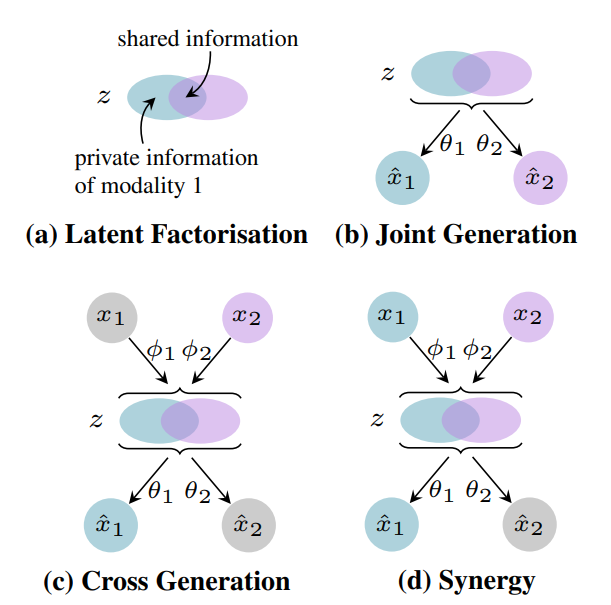
\includegraphics[scale=0.4]{figures/criteria.png}
    \caption{Criteria for Multimodal Generation \cite{MMVAE}}
    \label{fig:criteria}
\end{figure}

\ac{mmvae} proposed by \cite{MMVAE} fulfills all 4 of the above-mentioned criteria learning representations of image and text data, while other approaches focus on leveraging specific advantages of multimodal learning. Consider the cross-modal learning for 3D Hand Pose Estimation proposed by \cite{crossmodal}. It involves training an encoder-decoder pair to learn image representation, and another such pair to learn 3D hand pose representations in the same latent space. This training procedure focuses on cross-generation and synergy. That is, using the shared latent space of the image and pose representations, the \ac{rgb} image encoder combined with the pose decoder can generate 3D poses and vice versa while preserving the commonality between the conditioned and the generated data. With this approach, it is possible to train a \ac{vae} for 3D \ac{hpe} from \ac{rgb} images without explicit intermediate stages like the earlier mentioned cascading approaches. Making it more efficient and fast for both training and inference without compromising the modularity offered by cascading approaches.

% TODO -- Add more on non supervised learning papers
\section{Related Work - A closer look}
\label{section:Related Work}
\lipsum[1-5] %FIXME
